\documentclass{ecai}
\usepackage{times}
\usepackage{graphicx}
\usepackage{latexsym}
\usepackage{amsmath}
\usepackage{algorithm}
\usepackage{algorithmicx}
\usepackage{amsfonts}
\usepackage{bm}
%%\ecaisubmission   % inserts page numbers. Use only for submission of paper.
                  % Do NOT use for camera-ready version of paper.

\begin{document}

%\title{Guidelines for Preparing a Paper for the \\
%European Conference on Artificial Intelligence}
\title{Synthesis of Registered Brain Multimodal\\
	MRI with Lesions}
\author{ Yili Qu \and Wanqi Su \and Chufu Deng \and Ying Wang \\
	\and Yutong Lu \and Zhiguang Chen \and Nong Xiao \institute{Sun Yat-sen University,
China, email: quyli@mail2.sysu.edu.cn} }
\maketitle
\bibliographystyle{ecai}

\begin{abstract}
  In a large number of data-driven medical image intelligent processing tasks, the collection and acquisition of medical image data is very difficult, especially registered multimodal medical image data. Synthetic medical image data can alleviate the problem of insufficient data well. In this paper, based on the unsupervised conditional GAN model, we achieve the synthesis of registered multimodal medical images from a random normal distribution matrix, and the corresponding lesion information can be efficiently generated based on the freely selected lesion label. 
% Quality control editor: Abbreviations and acronyms are typically defined the first time the term is used within the abstract and again in the main text and then used throughout the remainder of the manuscript. Please consider adhering to this convention. The target journal may have a list of abbreviations that are considered common enough that they do not need to be defined.
We conduct a number of validation experiments on BRATS2015 to verify that our synthetic MRI data can be used as pre-trained data or enhanced data in medical image intelligent processing tasks, and they can greatly improve the generalization ability of the model.
\end{abstract}

\section{INTRODUCTION}
%The traditional page limit for ECAI long papers is {\bf 7 (six)} pages
%in the required format. The traditional page limit for short
%submissions is {\bf 2} pages.
%
%However, these page limits may change from one ECAI to
%another. Consult the most recent Call For Papers (CFP) for the most
%up-to-date page limits.

MRI is a common medical imaging technique that has multiple modalities depending on the imaging parameters, such as T1 and T2. Different modalities have different reference values for doctors. To make accurate judgments, doctors often need multiple modal images for comparison. Moreover, in training and learning of medical image intelligent processing tasks, we often expect to obtain more modal images, such as medical image processing tasks based on CNNs\cite{86krizhevsky2012imagenet} or GANs\cite{25goodfellow2014generative}. 

When obtaining different modalities from the same part of the same patient through different imaging techniques, these modalities are considered to be registered if the imaging position and the viewing angle are identical. Compared with unimodal data, the registered multimodal image data can provide more information, support more complex application scenarios, meet the training data requirements of deep neural networks, and help to make intelligent diagnostic services more efficient and more reliable. For doctors, it takes longer to acquire images of different modalities and requires patient patience. For researchers of medical image intelligent processing tasks, multimodal MRI datasets are scarce, and the collection is very difficult, especially for rare disease data, for which registered data are even rarer, which makes many training tasks impossible. Therefore, the application of image synthesis technology to extend datasets, translate existing unimodal images to registered multimodal images, or synthesize registered multimodal images from a random noise matrix has a wide range of uses and far-reaching significance.

Before the popularity of GANs, researchers focused on existing medical image modalities translate to other modalities\cite{22burgos2015robust,33huang2017simultaneous,34vemulapalli2015unsupervised,36vannguyen2015crossdomain}. Since the powerful generation ability of the GAN has been demonstrated, there have been many studies on medical image translation based on GANs\cite{2zhang2018translating,20nie2017medical,35osokin2017gans,36vannguyen2015crossdomain,40kamnitsas2017unsupervised}. Many studies use GANs to achieve higher translation quality\cite{1zhao2018modular,5liang2018generative,6zhu2017unpaired,13choi2018stargan:}. Recent studies have performed translation on unregistered multimodal data\cite{2zhang2018translating,85joyce2017robust}.
The GAN has been gradually applied to various organs, such as brain MRI to CT translation\cite{20nie2017medical,40kamnitsas2017unsupervised}, retinal vascular annotation to image translation\cite{41costa2017towards}, and cardiac MRI to CT translation and segmentation using unsupervised CycleGAN\cite{6zhu2017unpaired,20nie2017medical}.
For multimodal image synthesis, \cite{84chartsias2018multimodal} implements multi-input and multi-output MRI synthesis, but registration is required for input multimodal data. \cite{85joyce2017robust} further implements an unregistered multi-input synthesis model, which can perform image synthesis from any subset of its input but limits the output to unimodal. \cite{66Miao2018dilated} studies medical image registration in depth. \cite{4shin2018medical} uses a GAN to synthesize brain tumor images to enhance data and anonymize data but requires additional training of the anatomical structure segmentation network.
In addition, \cite{41costa2017towards} implements the random generation of vascular annotation maps based on the idea of variational auto-encoder (VAE)\cite{87kingma2014auto-encoding} and then generates colour retinal images based on the vascular annotation maps.
Beyond the field of medical image processing, the research of multi-domain translation is very active\cite{1zhao2018modular,5liang2018generative,13choi2018stargan:,27isola2017image-to-image}.
In the field of medical image synthesis, there are many studies regarding two-modal translation synthesis\cite{2zhang2018translating,20nie2017medical,22burgos2015robust,34vemulapalli2015unsupervised,35osokin2017gans,36vannguyen2015crossdomain,40kamnitsas2017unsupervised}, but research on multimodal synthesis is rare\cite{84chartsias2018multimodal,85joyce2017robust,4shin2018medical}.

At present, there are various problems in the research of medical image synthesis, including the difficulty of expanding the number of modalities, the need to registered training data, the reliance on complex large networks, the inability to add or retain lesions, the inability to synthesize from random matrix, the need for additional training data, etc. 
%Therefore
To solve these problems, we design a registered multimodal MRI synthesis scheme based on  conditional generative adversarial networks (CGANs)\cite{70mirza2014conditional}. With an unsupervised learning method, the training data do not need to be registered. Our solution can receive a random normal distribution matrix as input to synthesize a set of registered multimodal MRI images with selected lesions. We perform multimodal brain MRI synthesis experiments with tumor segmentation labels on BRATS2015 and verify the effectiveness of lesion information and the availability of synthetic data in tumor lesion segmentation experiments. 

In general, our main work includes the following three aspects:

\begin{itemize}
	\item{Extraction and generation of structural feature map}
	
	We propose an extraction method for anatomical structure features of medical images. Without additional anatomical segmentation labels or label extraction training, structural feature maps can be extracted directly from arbitrary real images. We also train a structural feature map generator to generate structural feature maps from a multidimensional normal distribution. Thus, we can generate rich and diverse structural feature maps indefinitely.
	
	\item{Synthesis of registered multimodal MRI with lesions}	
	
	We use randomly generated structural feature maps to fuse with random lesion labels and then synthesize the registered multimodal MRI through the generator. We explore a variety of lesion generation guidance methods to achieve effective mapping of lesions based on input lesion labels during multimodal MRI synthesis. In training, no registered data are required except for the lesion labels. 
	
	\item{Objective verification for synthetic data availability}
	
	We construct datasets with different quantities of synthetic and real data to train the lesion segmentor and verify that the synthetic data can be used as pre-training data and enhanced data in medical image intelligent processing tasks to improve generalization ability of the model and improve the segmentation precision. Therefore, we can present the availability of synthetic data in intelligent lesion processing tasks objectively.
\end{itemize}

\section{METHOD}
\label{method}
We apply our scheme to a multimodal brain MRI synthesis task, in which the synthetic lesions are tumors, the lesion processing task is lesion segmentation, and the lesion label is a tumor segmentation label. Our scheme does not limit the body parts, lesion types, lesion processing tasks, specific modality and the number of modalities. We can easily apply this method to other similar tasks. For more details on our method, refer to the open source code we provide.

\subsection{Architecture}
\begin{figure*}[t]
	\centering
	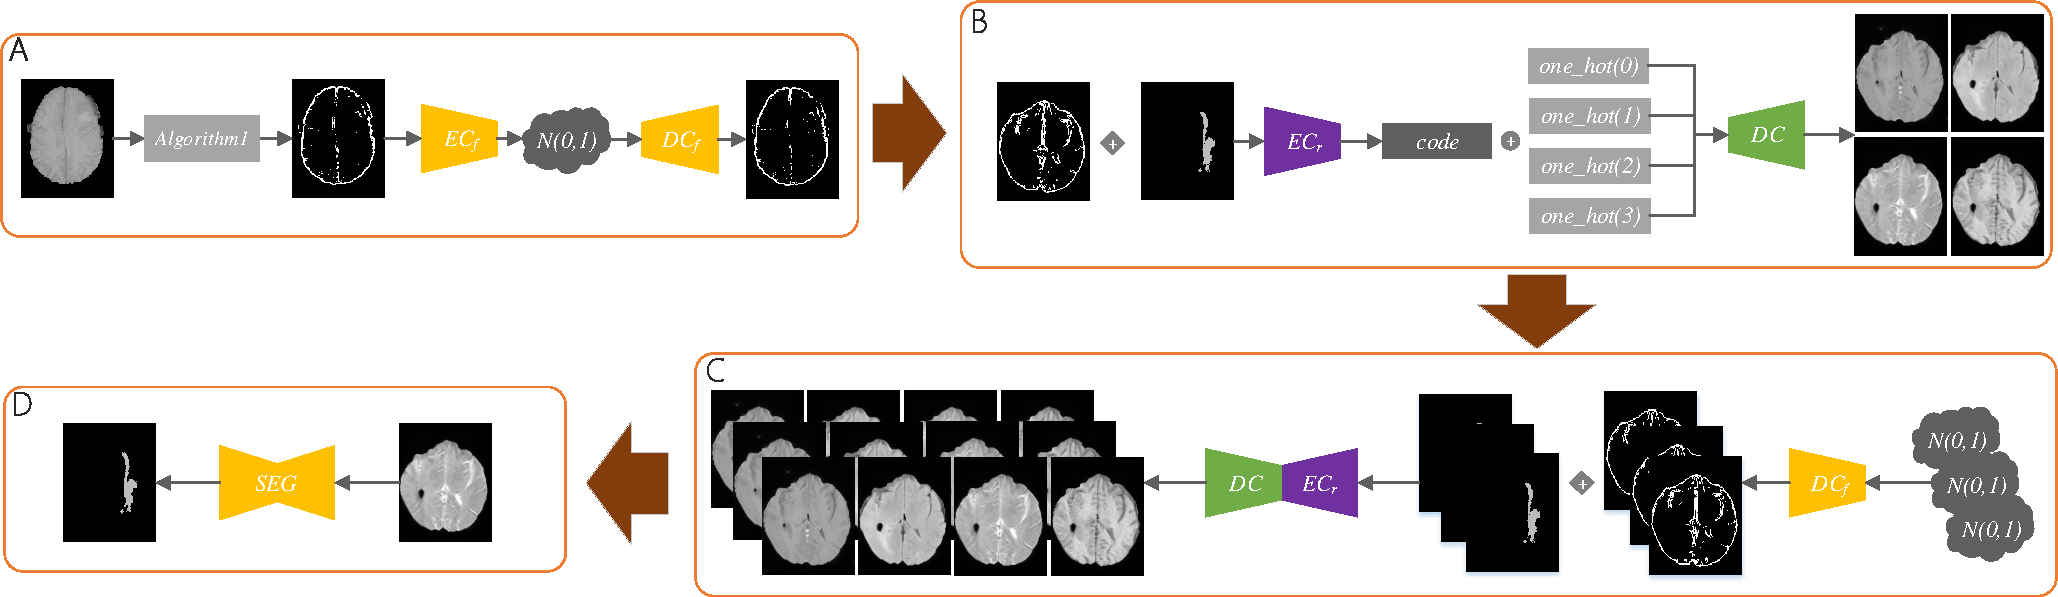
\includegraphics[width=0.85\textwidth]{figures/architecture}
	\caption{The overall architecture. A is the structural feature map extraction and generation stage. B is the multimodal MRI synthesis stage. C is the synthetic datasets construction stage. D is the synthetic data availability verification stage.}
	\label{architecture}
\end{figure*}
As shown in Fig.~\ref{architecture}, our scheme includes four main stages. 
\iffalse
In the structural feature map extraction and generation stage, we will obtain a structural feature map generator that can generate structural feature maps from a random normal distribution matrix. 
In the multimodal MRI synthesis stage, we train a conditional generator with input of structural feature maps and lesion labels, which can synthesize MRI images of different modalities according to different conditionals.
In the synthetic datasets construction stage, we use the models produced in the previous stages to synthesize registered multimodal MRI images from random normal distribution matrixes. 
In the synthetic data availability verification stage, we train and test the lesion segmentors on different datasets constructed from different quantities of synthetic data and real data.
\fi
In stage A, we obtain a structural feature map generator that can generate structural feature maps from a random normal distribution matrix. 
In stage B, we train a conditional generator with input of structural feature maps and lesion labels, which can synthesize MRI images of different modalities according to different conditionals.
In stage C, we use the models produced in the previous stages to synthesize registered multimodal MRI images from random normal distribution matrixes. 
%These three stages are performed in sequence and are indispensable, so we verify the availability of synthetic data in phase D.
In stage D, we train and test the lesion segmentors on different datasets constructed from different quantities of synthetic data and real data.
Limited by memory capacity, the network structure of each model component is simple multi-layer convolution with ReLU activation and instance normalization, and specifically described in the source code we provide. 

\subsection{Generation of structural feature map}
Medical images generated directly from random noise by GAN are difficult to generate realistic structural information. We call the image that provides basic contour and structure information a structural feature map. For example, a retinal vascular distribution map can be regarded as a structural feature map of a retinal image\cite{41costa2017towards}. Structural feature maps can provide necessary basic guidance for the synthesis of medical images. When synthesizing brain MRI images, some studies obtain basic structural information from the brain segmentation labels\cite{4shin2018medical}. However, general structural features such as retinal vascular maps and brain segmentation labels require additional data and training before extracting from the original image. To solve these problems, we first design a method for extracting structural feature maps directly from brain MRI images, which has the advantages of fast operation, no training, and no additional required data. Then, we train a generator to generate structural feature maps from random normal distribution matrixes.

\subsubsection{Structural feature map extraction method}
In the traditional digital image processing methods, the Roberts operator, Prewitt operator, Sobel operator, etc., are excellent edge detection operators. The Sobel operator is often used in the processing of brain medical images.
% As shown in Algorithm~\ref{alg:1}, we explore a method to further extract structural feature maps from the edge detection maps generated by Sobel operator.
\begin{algorithm}
	\caption{Structural feature map extraction}
	\label{alg:1}
	\begin{algorithmic}[1]
		\State Input a real image $x$ and pixel threshold $beta$
		\State $s1 = reduce\_min(sobel(x))$
		\State $s2 = reduce\_max(sobel(x))$
		\State $s1 = mean(s1) - s1$
		\State $s2 = s2 - mean(s2)$
		\State $s1 = ones \times (s1 > beta)$
		\State $s2 = ones \times (s2 > beta)$
		\State $s = ones \times ((s1 + s2)> 0.)$
	\end{algorithmic}  
\end{algorithm}
%In Algorithm~\ref{alg:1}
As shown in Algorithm~\ref{alg:1}, we use the Sobel operator to extract the horizontal and vertical edge detection maps from a real image. Each edge detection map performs maximum reduce and minimum reduce to obtain two edge detection fusion maps. Then, each fusion map calculates the difference from the average pixel value. The two difference maps are binarized according to the pixel threshold, and the two binary images are summed and then completely binarized. The final result is the structural feature map that we need.

\subsubsection{Structural feature map generation training}
\begin{figure}
	\centering
	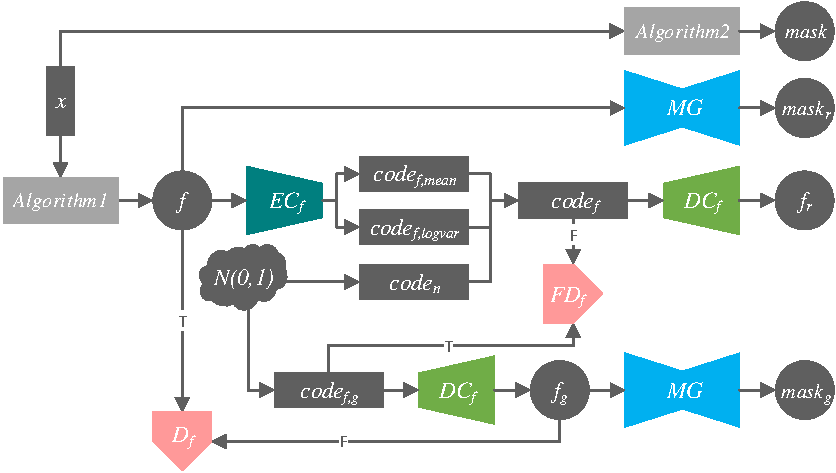
\includegraphics[width=0.98\columnwidth]{figures/feature_train}
	\caption{Structural feature map generation training. $x$ is an input real MRI image, $s$ is a structural feature map. $E_s$ is a VAE encoder, which outputs the encode matrixs $f_{mean}$ and $f_{logvar}$. $z$ is a random noise sampling from multidimensional normal distribution $\mathcal{N}(0,1^2)$ and the $f$ is a approximate normal distribution matrix. $G_s$ is a VAE decoder, $s_r$ is a reconstructed structural feature map, and $s_g$ is a generated random structure feature map. $D_{s}$ is a structural feature discriminator. $G_m$ is a mask generator and $m_r$ is a extracted mask. }
	\label{feature_train}
\end{figure}
\begin{algorithm}
	\caption{Mask Extraction}
	\label{alg:2}
	\begin{algorithmic}[1]
		\State Input a real image $x$ and the expanded pixel value $p$
		\State $m = 1.0 - ones \times (x > 0.)$
		\State $new\_size=[x.width() + p, x.length() + p]$
		\State $m = resize(m, new\_size)$
		\State $m = crop\_padding(m,p)$
	\end{algorithmic}  
\end{algorithm}
When generating the structural feature map, \cite{4shin2018medical} still needs to input the real image to obtain the generated structural feature map, which greatly reduces the diversity of the synthetic data. \cite{41costa2017towards} implements a method based on VAE for generating retinal blood vessel distribution maps from a multidimensional normal distribution. Drawing on this approach, we design a hybrid network combining the characteristics of VAE and GAN for generating brain structural feature maps from random normal distribution matrixes, which has better diversity and no additional training data. In addition, we train a generator $G_m$ that acquires the brain area masks from the brain structure feature maps for later use to match lesion labels. $G_m$ is synchronized with the training of structural feature map generation. During the training of $G_m$, the mask extracted using Algorithm~\ref{alg:2} is used as the label data. As shown in Fig.~\ref{feature_train}, the specific training processing is as follows:
\begin{itemize}
	\item The structural feature map $s$ is obtained from $x$ by using Algorithm~\ref{alg:1}. .
	\item Encode $s$ with VAE encoder $E_s$ to obtain $f_{mean}$ and $f_{logvar}$. Then, obtain the random noise $z$ from multidimensional normal distribution $\mathcal{N}(0,1^2)$ so that the approximate normal distribution matrix  $f=f_{mean}+exp(0.5\times f_{logvar})\times z$;
	\item Decode $f$ with VAE decoder $G_s$ to obtain the reconstructed structural feature map $s_r$;
%	\item Randomly generate a matrix $z$ that obeys normal distribution $\mathcal{N}(0,1^2)$;
	\item Decode the random noise $z$ with VAE decoder $G_s$ to obtain the generated random structure feature map $s_g$;
	\item Structural feature discriminator $D_{s}$ identifies $s$ and $s_g$, the former is a positive sample, and the latter is a negative sample;
	\item Train the mask generator $G_m$ to extract mask $m_r$ from $s$, and the mask $m$ obtained from $x$ by Algorithm~\ref{alg:2} is the trainnig label.
\end{itemize}

%For the constraint of approximate normal distribution matrix, we do not use the original VAE encoder loss but rather add a code matrix distribution discriminator to provide adversarial loss for VAE encoder. Meanwhile, we use the $L2$ regular loss to guide the mean matrix with a mean of 0 and the variance deviation matrix with a mean of 1.
The loss items are as follows, where $\mathbb{E}$ is the expectation operator: 
\begin{itemize}
	\item{Part A: Structural feature map reconstruction loss} 
	\begin{equation}
	\mathcal{L}_{r}(E_s,G_s)=\mathbb{E}_{s,f}[\Vert{s-s_r}\Vert_{2}^{2}],
	\end{equation}
	where $s_r=G_s(f)$.
%	where $s_r=G_s(f)$.	
%	\item{Code matrix distribution discriminator loss} 
%	\begin{equation}
%		\mathcal{L}_{1}(D_{c})=\mathbb{E}_{z,x}[\Vert{D_{c}( z_s)-1}\Vert_{2}^{2}+\Vert{D_{c}(V(x))}\Vert_{2}^{2}].
%	\end{equation}
	\item{Part B: Structural feature map discriminator and generator loss} 
	\begin{equation}
		\mathcal{L}_{d1}(D_{s})=\mathbb{E}_{s,z}[\Vert{D_{s}(s)-1}\Vert_{2}^{2}+\Vert{D_{s}(s_g)}\Vert_{2}^{2}],
	\end{equation}
	\begin{equation}
	\mathcal{L}_{g}(E_s,G_s)=\mathbb{E}_{z}[\Vert{D_{s}(s_g)-1}\Vert_{2}^{2}],	
	\end{equation}
	where $s_g=G_s(z)$.
%	\item{Structural feature map adversarial loss} 
%
%	\begin{equation}
%		\mathcal{L}_{3}(H,G)=\mathbb{E}_{z,x}[\Vert{D_{c}(V(x)-1}\Vert_{2}^{2}+\Vert{D_{s}(G(z))-1}\Vert_{2}^{2}].
%	\end{equation}
%	
%	\item{Code matrix distribution loss } 
%	\begin{equation}
%	\begin{split}
%	\mathcal{L}_{4}(H,G)=\mathbb{E}_{z_{f,mean},z_{f,logvar}}[\Vert{mean(z_{f,mean})}\Vert_{2}^{2}\\+\Vert{mean(exp(0.5\times z_{f,logvar}))-1}\Vert_{2}^{2}].
%	\end{split}
%	\end{equation}
	\item{Part C: Mask reconstruction loss}
	\begin{equation}
	\mathcal{L}_{m}(G_m)=\mathbb{E}_{m,s}[\Vert{m-m_r}\Vert_{2}^{2}],
	\end{equation}
	where $m_r=G_m(s)$.
\end{itemize}

\subsection{Multimodal MRI synthesis}
In this section, we use the fusion of the structural feature maps and randomly selected lesion labels as our fusion map encoder's input to eventually generate a wide variety of registered multimodal MRI. What's more, we conduct translation training on real MRIs to ensure that each component plays a specific role without confusion.
%\subsubsection{Fusion of structural feature map and label}
%After generating structural feature map $f_g$, we randomly select appropriate lesion segmentation label $label$, and the lesion segmentation label containing $n$ categories is converted into a one-hot matrix $onehot_l$ of $n$ channels. 
%%Each channel corresponds to a segmentation category, the pixel value in each channel is 0 or 1. Each 1 pixel area is registered with each original label segmentation area. 
%Then, we calculate the weighted sum of each channel of $onehot_l$ with $f_g$ and obtain a new matrix that fuses information of $f_g$ and $label$.
%
%If the structural feature map $f'$ is extracted from random MRI image $x$, then the extracted structural features may contain tumor structure information, which may interfere with the tumor information of random label $l$ and affect the synthetic MRI image; thus, $f'$ needs to eliminate the tumor information before fusing with random label $label$ and then obtain the structural feature map $s$ without tumor information, such that the tumor information of the synthetic image is only derived from label $label$. We generate a mask without boundary expansion $mask_{l,x}$ for segmentation label $label_x$ of $x$ by Algorithm~\ref{alg:2}; then, we have $f=mask_{l,x}\times f'$.
%
%Since the location of randomly selected lesion may appear outside the brain contour of structural feature map, we need to use Algorithm~\ref{alg:2} to obtain the brain region mask $m$ of structural feature map. If the product of $m$ and selected $label$ is 0, then the tumor label pixel is inside the brain contour of $m$, which can be adopted; otherwise, the $label$ needs to be re-selected.
\begin{figure*}
	\centering
	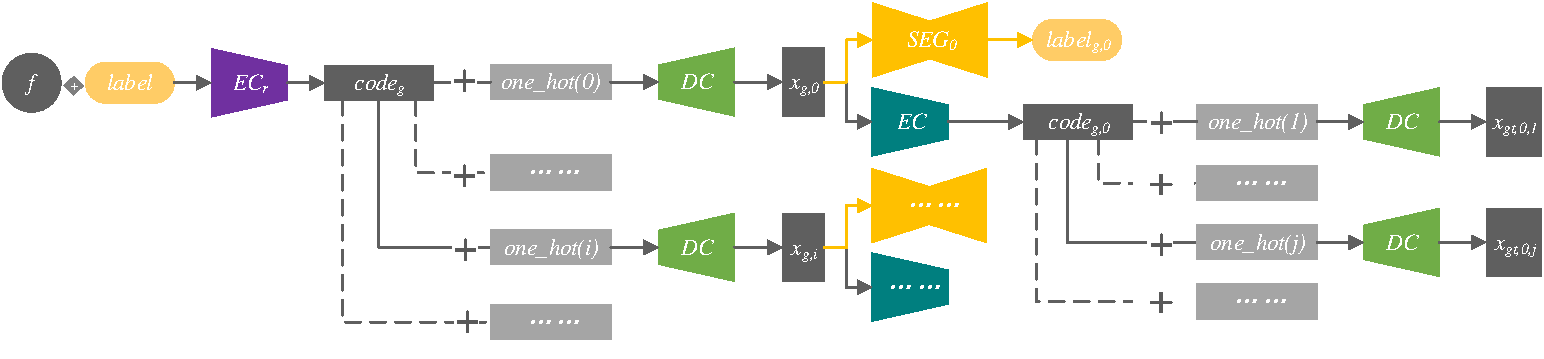
\includegraphics[width=1.98\columnwidth]{figures/mm_mri_generate}
	\caption{Synthesis of multimodal MRI images.
		 $s$ is a structural feature map and $l$ is a randomly selected real lesion label. $E$ is a fusion map encoder, which outputs the semantic feature map $f_g$, and  $i$ is a one-hot matrix stand for modality $i$. $G$ is a decoder and $x$ is MRI image. $G_{l,i}$ is a segmentor of modality $i$ and $E_x$ is an encoder.$x_{gt,i,j}$ is the synthetic image of the modality $j$ translated by synthetic image of modality $i$, $f_g$ is the semantic feature map obtained by fusion map encoder $E$, $f_{g,i}$ is the semantic feature map encoded from $x_i$. $l_{g,i}$ is the label obtained by lesion label generation component from $x_{g,i}$.
	}
	\label{mm_mri_generate}
\end{figure*}
\subsubsection{Multimodal MRI synthesis training}
\begin{figure*}
	\centering
	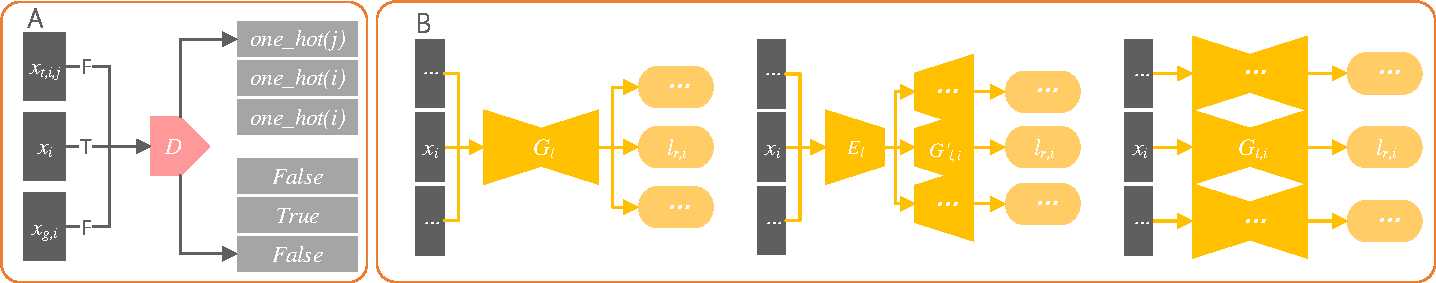
\includegraphics[width=1.98\columnwidth]{figures/DandSEG}
	\caption{A: Discriminator training on real MRI images and synthetic MRI image. B: Lesion segmentation training.}
	\label{train_D}
	\label{segmentation}
\end{figure*}
As shown in Fig.~\ref{mm_mri_generate}, first, we extract the structural feature map $s$ from real MRI images via Algorithm~\ref{alg:1} and randomly select the lesion label $l$ for fusion by concatenation. Since the location of randomly selected lesion may appear outside the brain contour of structural feature map, we need to use the brain region mask $m$ to filter the lesion label. If the tumor label pixel is inside the brain contour of $m$, then the $l$ can be adopted; otherwise, the $l$ needs to be re-selected. The fusion map contains basic anatomical information and lesion information of the target site. Then, we use a fusion map encoder $E$ to encode fusion map and obtain the semantic feature map $f_g$. $f_g$ is concatenated to different one-hot conditional matrixes as input to MRI decoder $G$ and then obtains a synthetic image of different modalities $x_{g,i}$. These synthetic images are then performing modal translation process between each other by MRI encoder $E_x$ and MRI decoder $G$. We use adversarial loss and category guidance loss provided by the MRI discriminator $D$ to constrain the synthetic image to approximate a real MRI image and constrain the consistency of all semantic feature maps and translation images by loss, thus ensuring the mutual registration of synthetic multimodal MRI images. 
In addition, we use the lesion label generation components $G_{l,i}$ to segment the tumor lesion segmentation labels from each synthetic MRI image to ensure that the synthetic multimodal images have synthesized corresponding lesion content based on the input lesion label. As Fig.~\ref{trans_train} shows, $G_{l,i}$ are only trained by real data in translation training of the following subsections. 

%What's more, we also use a code matrix distribution discriminator $FD$ to guide the consistency of code matrixes distribution between the two training processes. 
The discriminator is updated independently, and its training process is shown in Fig.~\ref{train_D} A, 
where $d(x_{i})$ and $c(x_{i})$ are the true/false discrimination and category discrimination of the discriminator $D(x_i)$, $d(x_{g, i})$ and $c(x_{g,i})$ are the output of $D(x_{g,i})$, $x_{g,i}$ is the synthetic image of modality $i$. 

The specific loss items are as follows:
\begin{itemize}
	\item{Discriminator loss }
	\begin{equation}
	\begin{split}
	\mathcal{L}_{d2}(D)=\mathbb{E}_{x,s,l}[\sum\limits_{i=0}(\Vert{d(x_i)-1}\Vert_{2}^{2}+\Vert{d(x_{g,i})}\Vert_{2}^{2}+\\
	\Vert{c(x_i)-i}\Vert_{2}^{2}+\Vert{c(x_{g,i})-i}\Vert_{2}^{2})],
	\end{split}
	\end{equation}
	where $x_{g,i}=G(f_g,i),f_g=E(s,l)$.
	\item{Adversarial and category guidance loss}
	\begin{equation}
		\mathcal{L}_{g2}(E,G)=\mathbb{E}_{s,l}[\sum\limits_{i=0}(\Vert{d(x_{g,i})-1}\Vert_{2}^{2}+\Vert{c(x_{g,i})-i}\Vert_{2}^{2})].
	\end{equation}
	\item{Lesion generation loss}
	\begin{equation}
		\mathcal{L}_{les}(E,G)=\mathbb{E}_{s,l}[\sum\limits_{i=0}(\Vert{l-l_{g,i}}\Vert_{2}^{2})],
	\end{equation}
	where $l_{g,i}=G_{l,i}(x_{g,i})$.
	\item{MRI registration loss}
	\begin{equation}
		\mathcal{L}_{reg}(E_x,G)=\mathbb{E}_{s,l}[\sum\limits_{j=0}\sum\limits_{i=0,i\neq j}(\Vert{x_{g,i}-x_{gt,j,i}}\Vert_{2}^{2})],
	\end{equation}
	where $x_{gt,i,j}=G(f_{g,i},j),f_{g,i}=E_x(x_{g,i})$.
	\item{Semantic consistency loss}
	\begin{equation}
	\begin{split}
		\mathcal{L}_{s}(G,E_x)=\mathbb{E}_{s,l}[\sum\limits_{i=0}(\Vert{f_g-f_{g,i}}\Vert_{2}^{2})\end{split}
	\end{equation}
	
\end{itemize}

\subsubsection{Translation and segmentation training on real MRIs}
As shown in Fig.~\ref{trans_train}, we perform segmentation and translation training on real data. These trianings constrain each component to complete our specified tasks in the multimodal MRI synthesis process.
In translation training, encoder $E_x$ encodes real MRI $x_i$ of modality $i$ to obtain semantic feature map $z_{i}$; then, it is concatenated into different conditional matrixes, and all the modalities are obtained through decoder $G$. In the cycle-reconstruction process, we use the encoder to re-encode all the obtained translation images, concatenate all re-encoded semantic feature maps with conditional vector of modality $i$, and finally decode them using the decoder to obtain cycle-reconstruction image $x_{rc,j,i}$. In segmentation training, we use the lesion label $l_i$ of original input modality $x_i$ as the supervised label for lesion generation training and use lesion label generation components for $x_i$ to obtain $l_{r,i}$. 
%%As shown in Fig.~\ref{trans_train}, when the MRI is reconstructed and translated, encoder $EC$ encodes real MRI $x_i$ of modality $i$ to obtain semantic feature map $z_{i}$, then it is concatenated to different conditional matrixes and obtain all the modalities through decoder $DC$. In cycle-reconstruction, we use encoder to re-encode all the obtained translation images, concatenate all re-encoded semantic feature maps with conditional vector of modality $i$, and finally decode them by decoder to get cycle-reconstruction image $x_{rc,j,i}$. In the above process, we use the lesion label $l_i$ of original input modality $x_i$ as the supervised label for lesion generation training, and use lesion label generation components for $x_i$ to get $l_{r,i}$. 

Except the adversarial loss and the cycle consistency loss in CycleGAN\cite{6zhu2017unpaired} and reconstruction self-supervision loss in translation training, there is a lesion segmentation loss item for the training of the segmentator $G_{l,i}$ :
\begin{equation}
\label{lesion segmentation loss}
\mathcal{L}_{les}(G_{l,i})=\mathbb{E}_{x,l}[\Vert{l_i-l_{r,i}}\Vert_{2}^{2}],
\end{equation}
where $l_{r,i}=G_l(x_{i})$.
%%We perform reconstruction and translation training on real data and synchronize with multimodal MRI synthesis training in subsequent sections. These trainings constrain each component to complete our specified tasks in the multimodal MRI synthesis process. In addition, we use a code matrix distribution discriminator $FD$ to guide the consistency of code matrixes distribution between the two training processes. All discriminator components are updated independently. The discriminator training process is shown in Fig.~\ref{train_D}.

\begin{figure*}
	\centering
	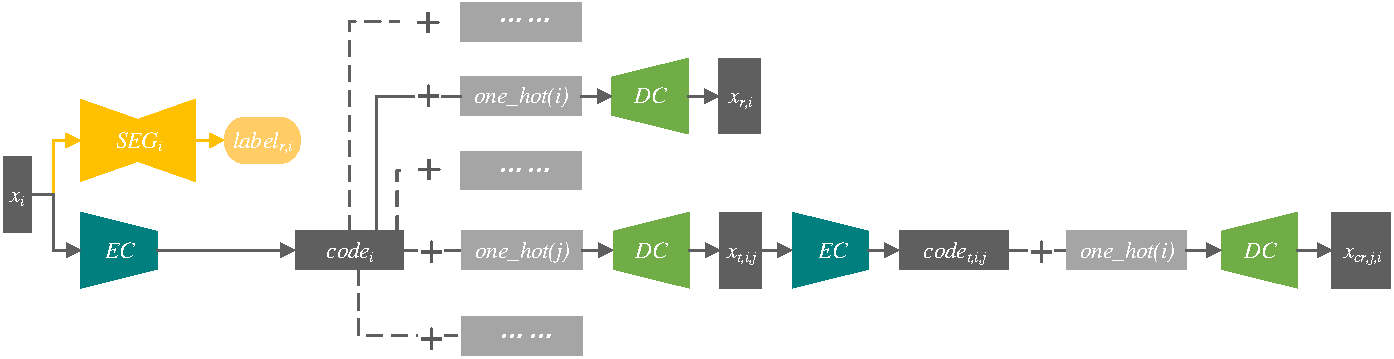
\includegraphics[width=1.75\columnwidth]{figures/trans_train}
	\caption{Translation and segmentation training on real MRIs.}
	\label{trans_train}
\end{figure*}

%%The detailed losses are as follows, where $x_{t,j,i}$ refers to MRI $x_i$ of modality $i$ translated by modality $j$, $d_{t, j, i}$ and $c_{t, j, i}$ are the true/false discrimination and category discrimination results of discriminator $D$ for $x_{t, i, j}$, and $z_{t,i,j}$ represents the semantic feature map obtained from $x_{t,i,j}$ by the encoder:
%\begin{itemize}
%%	\item{Feature Discriminator loss}
%%	\begin{equation}
%%	\begin{split}
%%	\mathcal{L}_{fd}=\sum\limits_{i=0}\Vert{FD(z_{i})-1}\Vert_{2}^{2}
%%	\end{split}
%%	\end{equation}
%	\item{Lesion segmentation loss}
%	\begin{equation}
%	\mathcal{L}_{les}(G_{l,i})=\mathbb{E}_{x,l}[\Vert{l_i-l_{r,i}}\Vert_{2}^{2}],
%	\end{equation}
%		where $l_{r,i}=G_l(x_{i})$.
%	
%\end{itemize}

\subsubsection{Lesion generation guidance method}
\label{label gen methods}
As shown in Fig.~\ref{segmentation} B, including the method mentioned above, we design the following three lesion label generation components to provide guidance loss for lesion generation in multimodal MRI image synthesis training:
\begin{enumerate}
	\item{Single segmentor} 
	
	Each MRI modality  is segmented by a common complete segmentor $G_l$.
	\item{Single lesion encoder + multiple lesion decoders} 
	
	Each MRI modality  is segmented by a segmentor, which comprises a common lesion encoder $E_{l}$ and different lesion decoders $G_{l,i}$. 
	\item{Multiple segmentors} 

	Each MRI modality  is segmented by a different complete segmentor $G_{l,i}$.
\end{enumerate}
The loss item of the above three methods in reconstruction and translation training is consistent with the loss item described above(Eq.~\ref{lesion segmentation loss}). In the generation training, it only provides the same lesion label generation loss for MRI synthesis components, i.e., there is no learning on synthetic MRIs.

%\begin{figure}
%	\centering
%	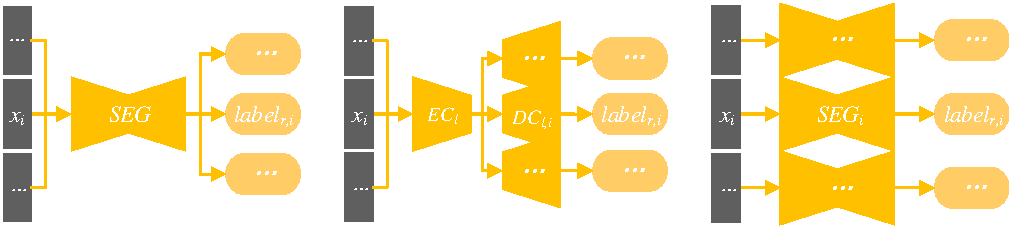
\includegraphics[width=0.98\columnwidth]{figures/segmentation}
%	\caption{Lesion segmentation.}
%	\label{segmentation}
%\end{figure}
%we train the segmentors of these three methods independently. In different experiments, we will train the segmentor in each method with different quantities of synthetic data or real data. The loss function of the training is as follows, where $l_i$ is the supervised label and $l_{r,i}$ is the segmentation result:
%\begin{equation}
%	\mathcal{L}_{segmentation}=\sum\limits_{i=0}\Vert{l_i-l_{r,i}}\Vert_{2}^{2}
%\end{equation}

\subsection{Construction of synthetic datasets}
\label{make dataset}
\begin{figure*}
	\centering
	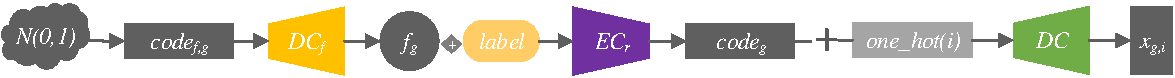
\includegraphics[width=1.78\columnwidth]{figures/make_data}
	\caption{Construction of synthetic datasets.}
	\label{make_data}
\end{figure*}
As shown in Fig.~\ref{make_data}, we can generate any number of structural feature maps from random normal distribution matrix through the trained structural feature map decoder. Then, we randomly scale, rotate, translate, and flip the original label set to obtain a random lesion label set. We then fuse the generated structural feature map with a randomly selected label from the random lesion label set. Like the training stage, we can select suitable labels by obtaining masks from structural feature maps through the mask generator $G_m$.

Due to the influence of the operation that removes the tumor region in input structural feature maps according to the label of the corresponding MRI in training stage, there are some structural feature maps with poor quality in which brain contour is not closed, so we design a structural feature map filtering algorithm for this purpose. First, we use the generator $G_m$ to generate the mask of the structural feature map. Then, we perform Gaussian blur\cite{92wink2004denoising} on the structural feature map and use the contour search algorithm and filling algorithm provided by OpenCV\footnote{https://opencv.org/} to obtain all the closed contours of the Gaussian blur image and fill them. Therefore, we obtain another mask by the traditional algorithm. Finally, we calculate the mean absolute error (MAE) of the two masks. If the MAE is less than the threshold we set, that means that the main brain contour of the structural feature map is relatively complete, and the feature map can be used; otherwise, it means that the mask obtained by the traditional algorithm is hollow inside and quite different from the mask generated by generator, so it needs to be regenerated. 
%The algorithm is expressed as Algorithm~\ref{alg:3}.
%\begin{algorithm}
%	\caption{Structural Feature Map Filtering}
%	\label{alg:3}
%	\begin{algorithmic}[1]
%		\State Input a MAE threshold $mae$
%		\State \textbf{function} $get\_mask(f)$
%		\State \indent$contours = OpenCV.findContours(f)$
%		\State \indent$mask =OpenCV.drawContours(f,contours)$
%		\State \indent\textbf{return} $m$
%		\State \textbf{do} 
%		\State \indent$f = G()$
%		\State \indent$m = G_m(f)$
%		\State \indent$m'= get\_mask(f)$
%		\State \textbf{while} $MAE(m',m) <= mae$
%	\end{algorithmic}  
%\end{algorithm}

In the synthetic multimodal MRI dataset, there are still samples with poor quality of lesion generation. At this point, we segment our synthetic MRI data through the lesion segmentor pre-trained on real data. We filter according to the segmentation evaluation score (the default threshold is 0.95 for the Dice score). After multiple filtering, we obtain the final synthetic dataset consisting of structural feature maps, masks, lesion segmentation labels, and multimodal MRI images.

\section{EXPERIMENTS}

\subsection{BRATS2015 dataset}
We use the open dataset BRATS2015\cite{91menze:hal-00935640} for experiments, which has four registered modalities of T1/T2/T1c/Flair. The training dataset contains 274 3D MRIs per modality, with the size of 155$\times$240$\times$240, and 274 tumor segmentation labels of the same size. We divide the sample into a training set and a test set by 9:1 and construct a 2D data set from 50 slices of each 55-105 of the 3D MRI. For data preprocessing, we standardize each image.

\subsection{BRATS synthetic dataset}
We construct a registered synthetic dataset with tumor labels containing four modalities of T1/T2/T1c/Flair using the method in Section~\ref{make dataset}. The sizes of the synthetic dataset samples are consistent with the BRATS2015 dataset, but the number of samples can be any number according to the needs of the experiment.

\subsection{BRATS enhanced dataset}
We perform random scaling, rotation, translation, flipping, etc. on the original BRATS2015 dataset to obtain enhanced data. The size of the enhanced dataset sample is consistent with the BRATS2015 dataset, but the number of samples can be any number according to the needs of the experiment.

\subsection{Training settings}
The iteration number of each experiment is equal to 100 epochs of the BRATS2015 training dataset. The learning rate is 1e-4 without weight decay. We use the Adam optimizer with beta1 of 0.5 and perform a dropout of 0.1 on the input layer; the batch size is 4. We use Dice score \cite{95dice1945measures} and mean square error (MSE)\cite{94prasad1990the} to evaluate the segmentation results. The evaluation results are the average of the 4 modal results on the 2D images, and each experiment is trained four times to retain the best results. For more details on training settings, refer to the source code we provided.

\subsection{Ablation experiments}
We perform simple ablation experiments to varify the effects of different components. We conduct experiment on replacing the structural feature map with random noise as input for MRI generation trainning. We conduct experiment by selecting input labels without mask limit. We conduct experiment on removing the translation training for registration on synthetic MRIs. We conduct experiment on removing the translation training on real MRIs. We conduct experiment on removing the lesion guidance loss in MRI synthesis training. The above 5 experiments are compared with our complete method.

\subsection{Experiments regarding lesion generation methods}
\label{label gen methods tests}
We train the segmentors of three methods in Section~\ref{label gen methods} independently. In different experiments, we will train the segmentor in each method with different quantities of synthetic data or real data. As shown in Table~\ref{label_test}, we train 4 tumor lesion segmentors using the multiple segmentors method on the BRATS2015 training dataset and test them on the BRATS2015 test dataset. Then, we use the trained segmentors to segment the unfiltered synthetic data from different lesion generation guidance methods.

\subsection{Experiments regarding synthetic data availability}
As shown in Table~\ref{availability_test}, we mix real BRATS2015 training data with BRATS synthetic data in different amounts, then use the mixed dataset for segmentation training using the multiple segmentors method, and finally evaluate the segmentation ability of the model on the real BRATS2015 test dataset. All experiments are fully trained with the same number of iterations, which is equal to the number of 100 epochs on the BRATS2015 training dataset. At the same time, we set up three data mixing modes: random mixing, real data training first, and synthetic data training first. In the real-first experiments and synthetic-first experiments, the training iteration number of data from different sources is proportional to the quantity of data. Except for the conditions listed in the table, the other conditions are identical.

\section{RESULTS}


\subsection{Results of ablation experiments}
Fig~\ref{ablation} shows examples of synthetic images generated in ablation experiments. 

\begin{figure}
	\centering
	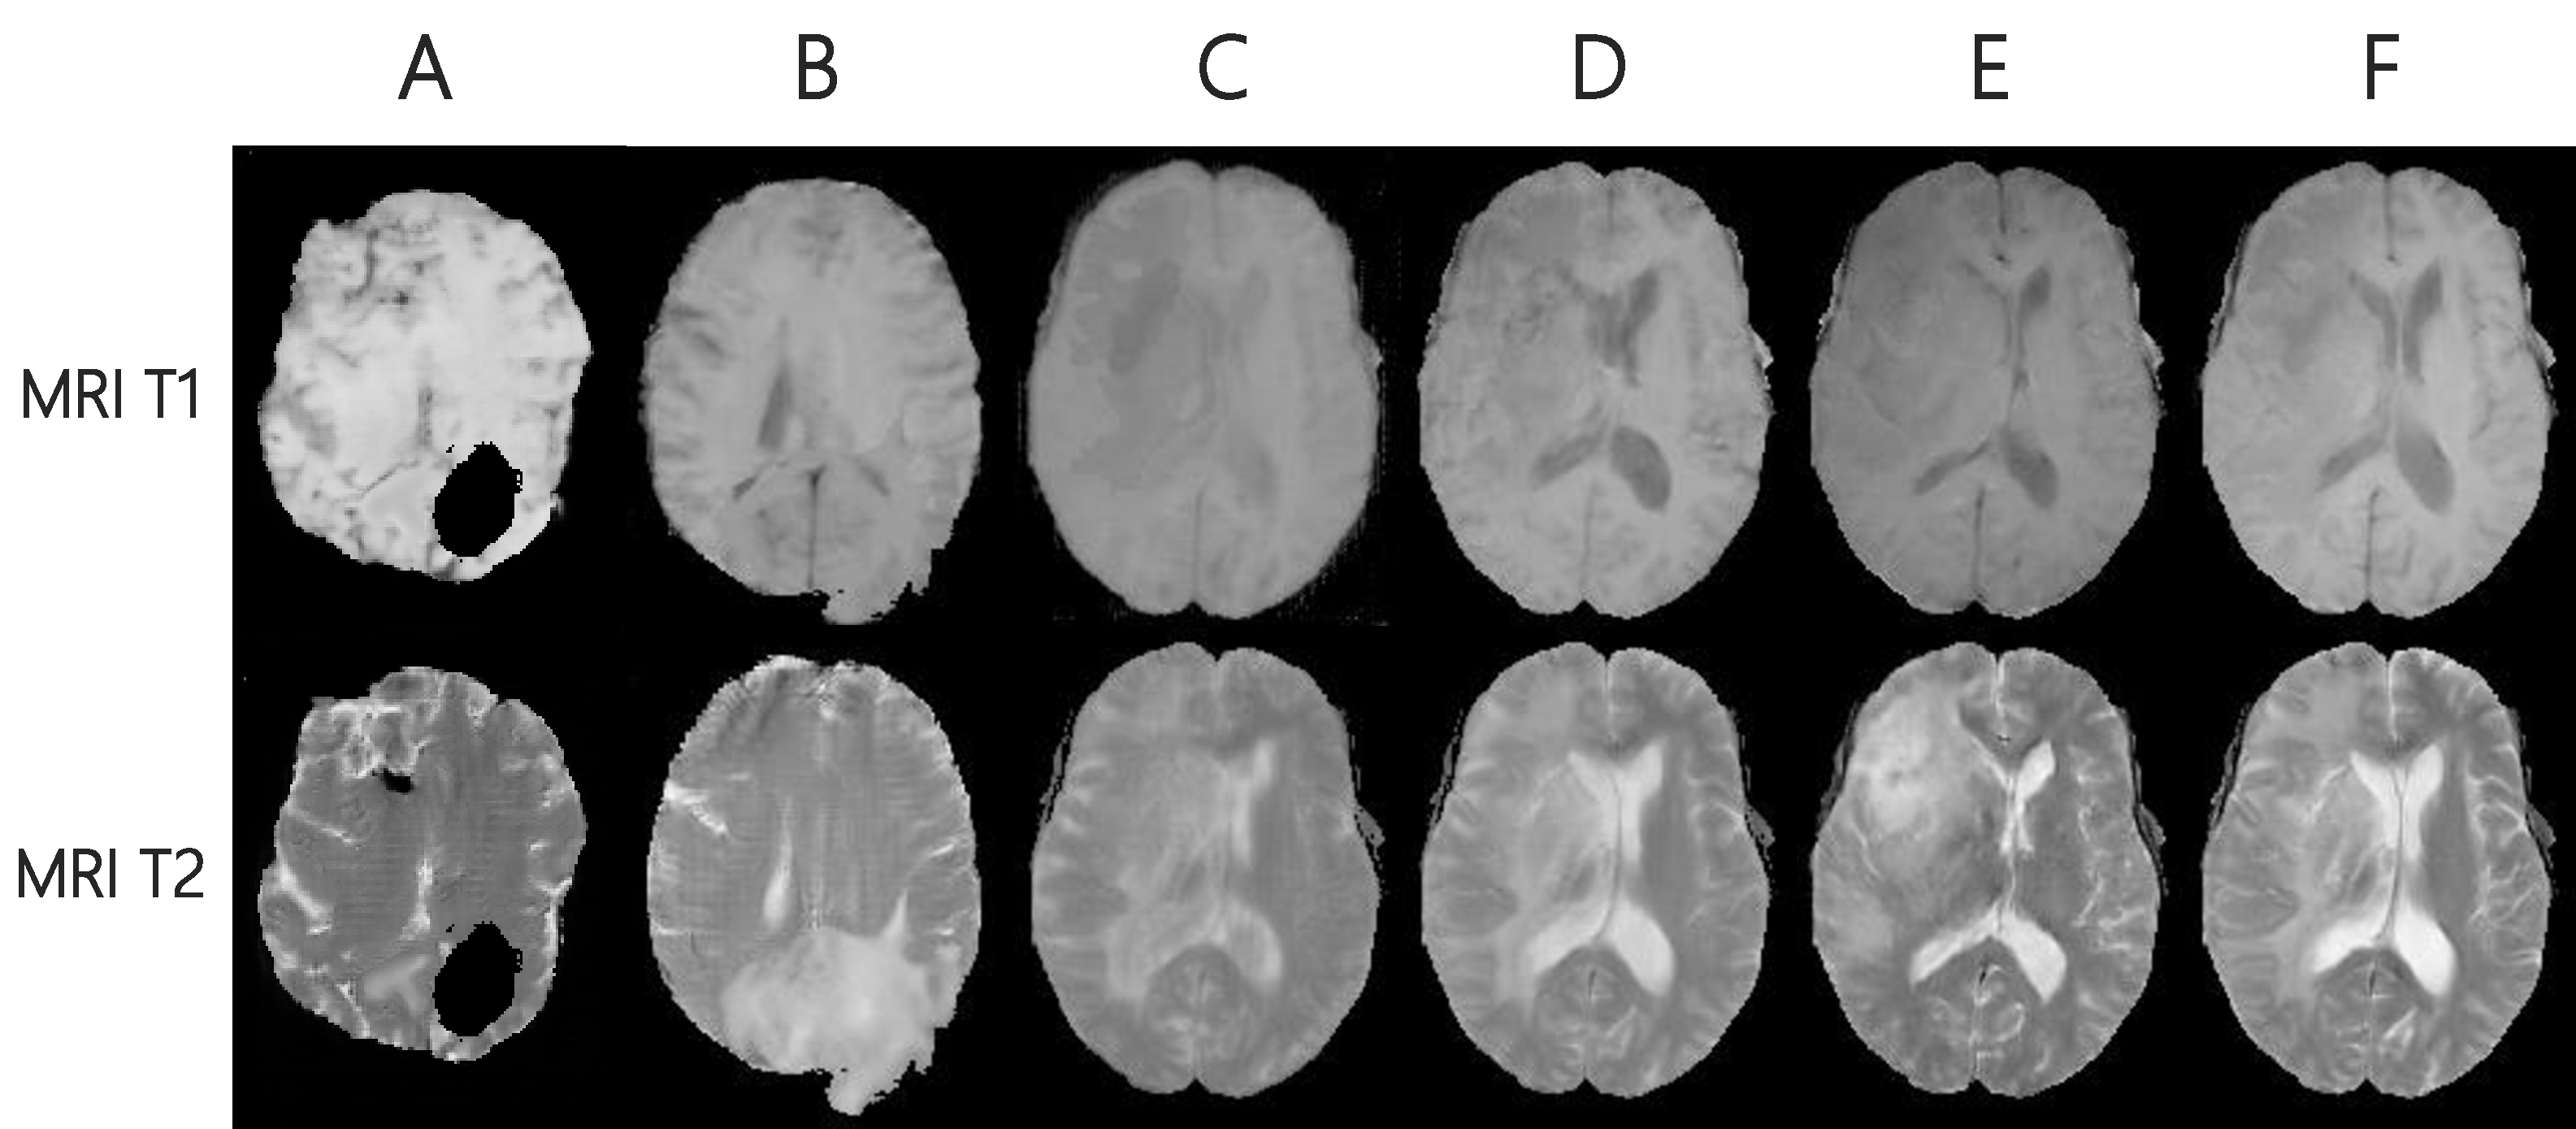
\includegraphics[width=0.98\linewidth]{figures/ablation}
	\caption{Synthetic images of ablation experiments. Model A: replace the structural feature map with random noise, without the constraint of the structural feature map on the brain contour, the image generated by model A conforms to the characteristics of MRI, but does not conform to the structural characteristics of the brain. Model B: remove the mask, it is easy to observe that the tumor generated by model B exceeds the contour of the brain. Model C: remove the translation training. Model D: remove the reconstruction training. The registration effect of the images generated by models C, D is not very good and the quality of the synthesis is not high. Model E: remove the lesion loss in multimodal MRI synthesis training process, it can be seen that the lesions in generated images do not correspond well to the input lesion label. Model F: our complete model.}
	\label{ablation}
\end{figure}

\subsection{Results of lesion generation methods}
\begin{table}
	\begin{center}
		{\caption{Lesion generation methods experiments.}\label{label_test}}
		\begin{tabular}{lcccc}
			\hline
			\rule{0pt}{12pt}
			segmentation schemes&testing dataset &MSE   &Dice score
			\\
			\hline
			\\[-6pt]
			\quad 4 $G_l$&real 		   				&0.026 &0.915 \\					
			\quad 1 $G_l$&synthetic     			&0.053 &0.741 \\			
			\quad 1 $E_{l}$ + 4 $D'_{l,i}$&synthetic     	&0.055 &0.808 \\		
			\quad 4 $G_{l,i}$&synthetic     			&\textbf{0.043} &\textbf{0.838} \\
			\hline
			\\[-6pt]
		\end{tabular}
	\end{center}
\end{table}
\begin{table}
	\begin{center}
		{\caption{Synthetic data availability verification experiments.}\label{availability_test}}
		\begin{tabular}{lllllcc}
			\hline
			\rule{0pt}{12pt}
			NO. &real &synthetic & enhanced & mix  & MSE &Dice score\\
			\hline
			\\[-6pt]
			\quad 1 & $\times$1  	 	& 0 		&0 			&- &0.026 &0.915 \\
			\quad2 & $\times$50\% 	 & 0  		&0 			&- &0.032 &0.902 \\
			\quad3 &0 	 	 & $\times$1  	&0 			&- &0.205 &0.708 \\
			\quad4 &0 	 	 & $\times$2  	&0 			&$\mathcal{M}$ &0.206 &0.736 \\
			\quad5 &0 		 & $\times$3  	&0 			&$\mathcal{M}$ &0.205 &0.754 \\
			\quad6 & $\times$10\% 	 & $\times$1  	&0 			&$\mathcal{S}$ &0.031 &0.908 \\
			\quad7 & $\times$10\% 	 & $\times$2   &0 			&$\mathcal{S}$ &0.028 &0.907 \\
			\quad8 & $\times$10\% 	 & $\times$3   &0 			&$\mathcal{S}$ &0.030 &0.907 \\	
			\quad9 & $\times$20\% 	 & $\times$80\% 	&0  		&$\mathcal{M}$ &0.041 &0.850 \\
			\quad10& $\times$50\% 	 & $\times$50\% 	&0  		&$\mathcal{M}$ &0.031 &0.904 \\
			\quad11& $\times$80\% 	 & $\times$20\% 	&0  		&$\mathcal{M}$ &0.024 &0.935 \\
			\quad12& $\times$1 	 	& $\times$20\% &0  		&$\mathcal{M}$ &0.025 &0.921 \\
			\quad13& $\times$1 	 	& $\times$50\% &0  		&$\mathcal{M}$ &\textbf{0.023} &\textbf{0.939} \\
			\quad14& $\times$1 	 	& $\times$80\% &0  		&$\mathcal{M}$ &0.026 &0.916 \\
			\quad15& $\times$1 	 	& $\times$1    &0   		&$\mathcal{M}$ &0.027 &0.913 \\
			\quad16& $\times$1 	 	& $\times$2   &0 			&$\mathcal{M}$ &0.033 &0.901 \\
			\quad17& $\times$1 	 	& $\times$3   &0 			&$\mathcal{M}$ &0.034 &0.897 \\	
			\quad18& $\times$1 	 	&0 		&  $\times$20\%	 	&$\mathcal{M}$ &0.027 &0.911 \\
			\quad19& $\times$1 	 	&0 		&  $\times$50\% 	&$\mathcal{M}$ &0.025 &0.927 \\
			\quad20& $\times$1    	&0 		&  $\times$80\% 	&$\mathcal{M}$ &0.026 &0.920 \\
			\quad21& $\times$1 	 	&0 		&  $\times$1    &$\mathcal{M}$ &0.026 &0.915 \\
			\quad22& $\times$1 	 	&0 		&  $\times$2   &$\mathcal{M}$ &0.032 &0.898 \\
			\quad23& $\times$1 	 	&0 		&  $\times$3   &$\mathcal{M}$ &0.036 &0.885 \\			
			\quad24& $\times$1 	 	& $\times$1 	&0  		&$\mathcal{R}$ &0.195 &0.795 \\
			\quad25& $\times$1 	 	& $\times$1 	&0  		&$\mathcal{S}$ &\textbf{0.021} &\textbf{0.940}
			\\
			\hline
			\\[-6pt]
			\multicolumn{7}{l}{$\mathcal{M}:$ random mixing\ \
				$\mathcal{S}:$ synthetic first\ \
				$\mathcal{R}:$ real first}
		\end{tabular}
	\end{center}
\end{table}
As reported in Table~\ref{label_test}, the segmentation test results of the segmentor trained on real data reach an MSE of 0.026 and Dice score of 0.915. From the results, three different lesion label generation methods have achieved good segmentation results, where the multiple segmentors method is the best. 

\subsection{Results of Synthetic Data Availability}
As reported in Table~\ref{availability_test}, the results of experiments NO.3-NO.5 show that the synthetic data cannot completely replace real data in training.           
The results of NO.6-NO.8 show that the performances of pre-training with a large quantity of synthetic data and fine-tuning on a small quantity of real data are similar to those of training with complete real data.  
In NO.9-NO.11, the results of different mixing ratios are also quite different. When the two ratios are close, the segmentation results are similar to those of NO.1. When the proportion of synthetic data is high, the synthetic data will interfere with the learning of real data, and the result is lower than that of NO.1. When the proportion of synthetic data is low, the generalization ability of the model can be improved by synthetic data, and the result is higher than NO.1.           
In NO.12-NO.17, we further try to add synthetic data of different quantities to real data, which show that adding a small quantity of synthetic data can enhance the learning and that the more synthetic data there are, the better the enhancement effect is; however, when the fraction of synthetic data reaches a certain percentage and then continues to increase, it achieves the opposite effect. 
In NO.18-NO.23, we compare the enhancement effect of synthetic data and enhanced data generated by usual data enhancement methods. We found that the two are similar but not equal in the trend between  enhancement effect and the increase in data quantity. Overall, the enhanced data are more robust in terms of the sensitivity of model to the quantity of enhanced data, but the enhancement effect upper limit of synthetic data is much higher than that of enhanced data.  
We compared NO.24-NO.25 with NO.15 and found that the performance of synthetic data is the best when they are used as pre-training data, and the performance is poor when they are used as supplementary training data. When using as enhanced data to mix with real data, the synthetic data can also achieve certain enhancements.

Generally, if there is a large quantity of real data, a small quantity of synthetic data can be used as enhanced data, or a large quantity of synthetic data can be used for pre-training and then training on real data. If there are fewer real data, a large number of synthetic data can be used for pre-training, and then, fine-tuning can be performed on a small quantity of real data, whose results can compete with the results on complete real data; this conclusion is consistent with \cite{4shin2018medical}. We do not recommend using synthetic data completely for training and also do not recommend using synthetic data for supplementary training.

\subsection{Results of Synthetic Data on All Stages}
Fig.~\ref{generated_f} shows examples of structural feature maps generated from random normal distribution matrixes. And Fig.~\ref{generated_mri} shows examples of images obtained from all stages.
\begin{figure}
	\centering
	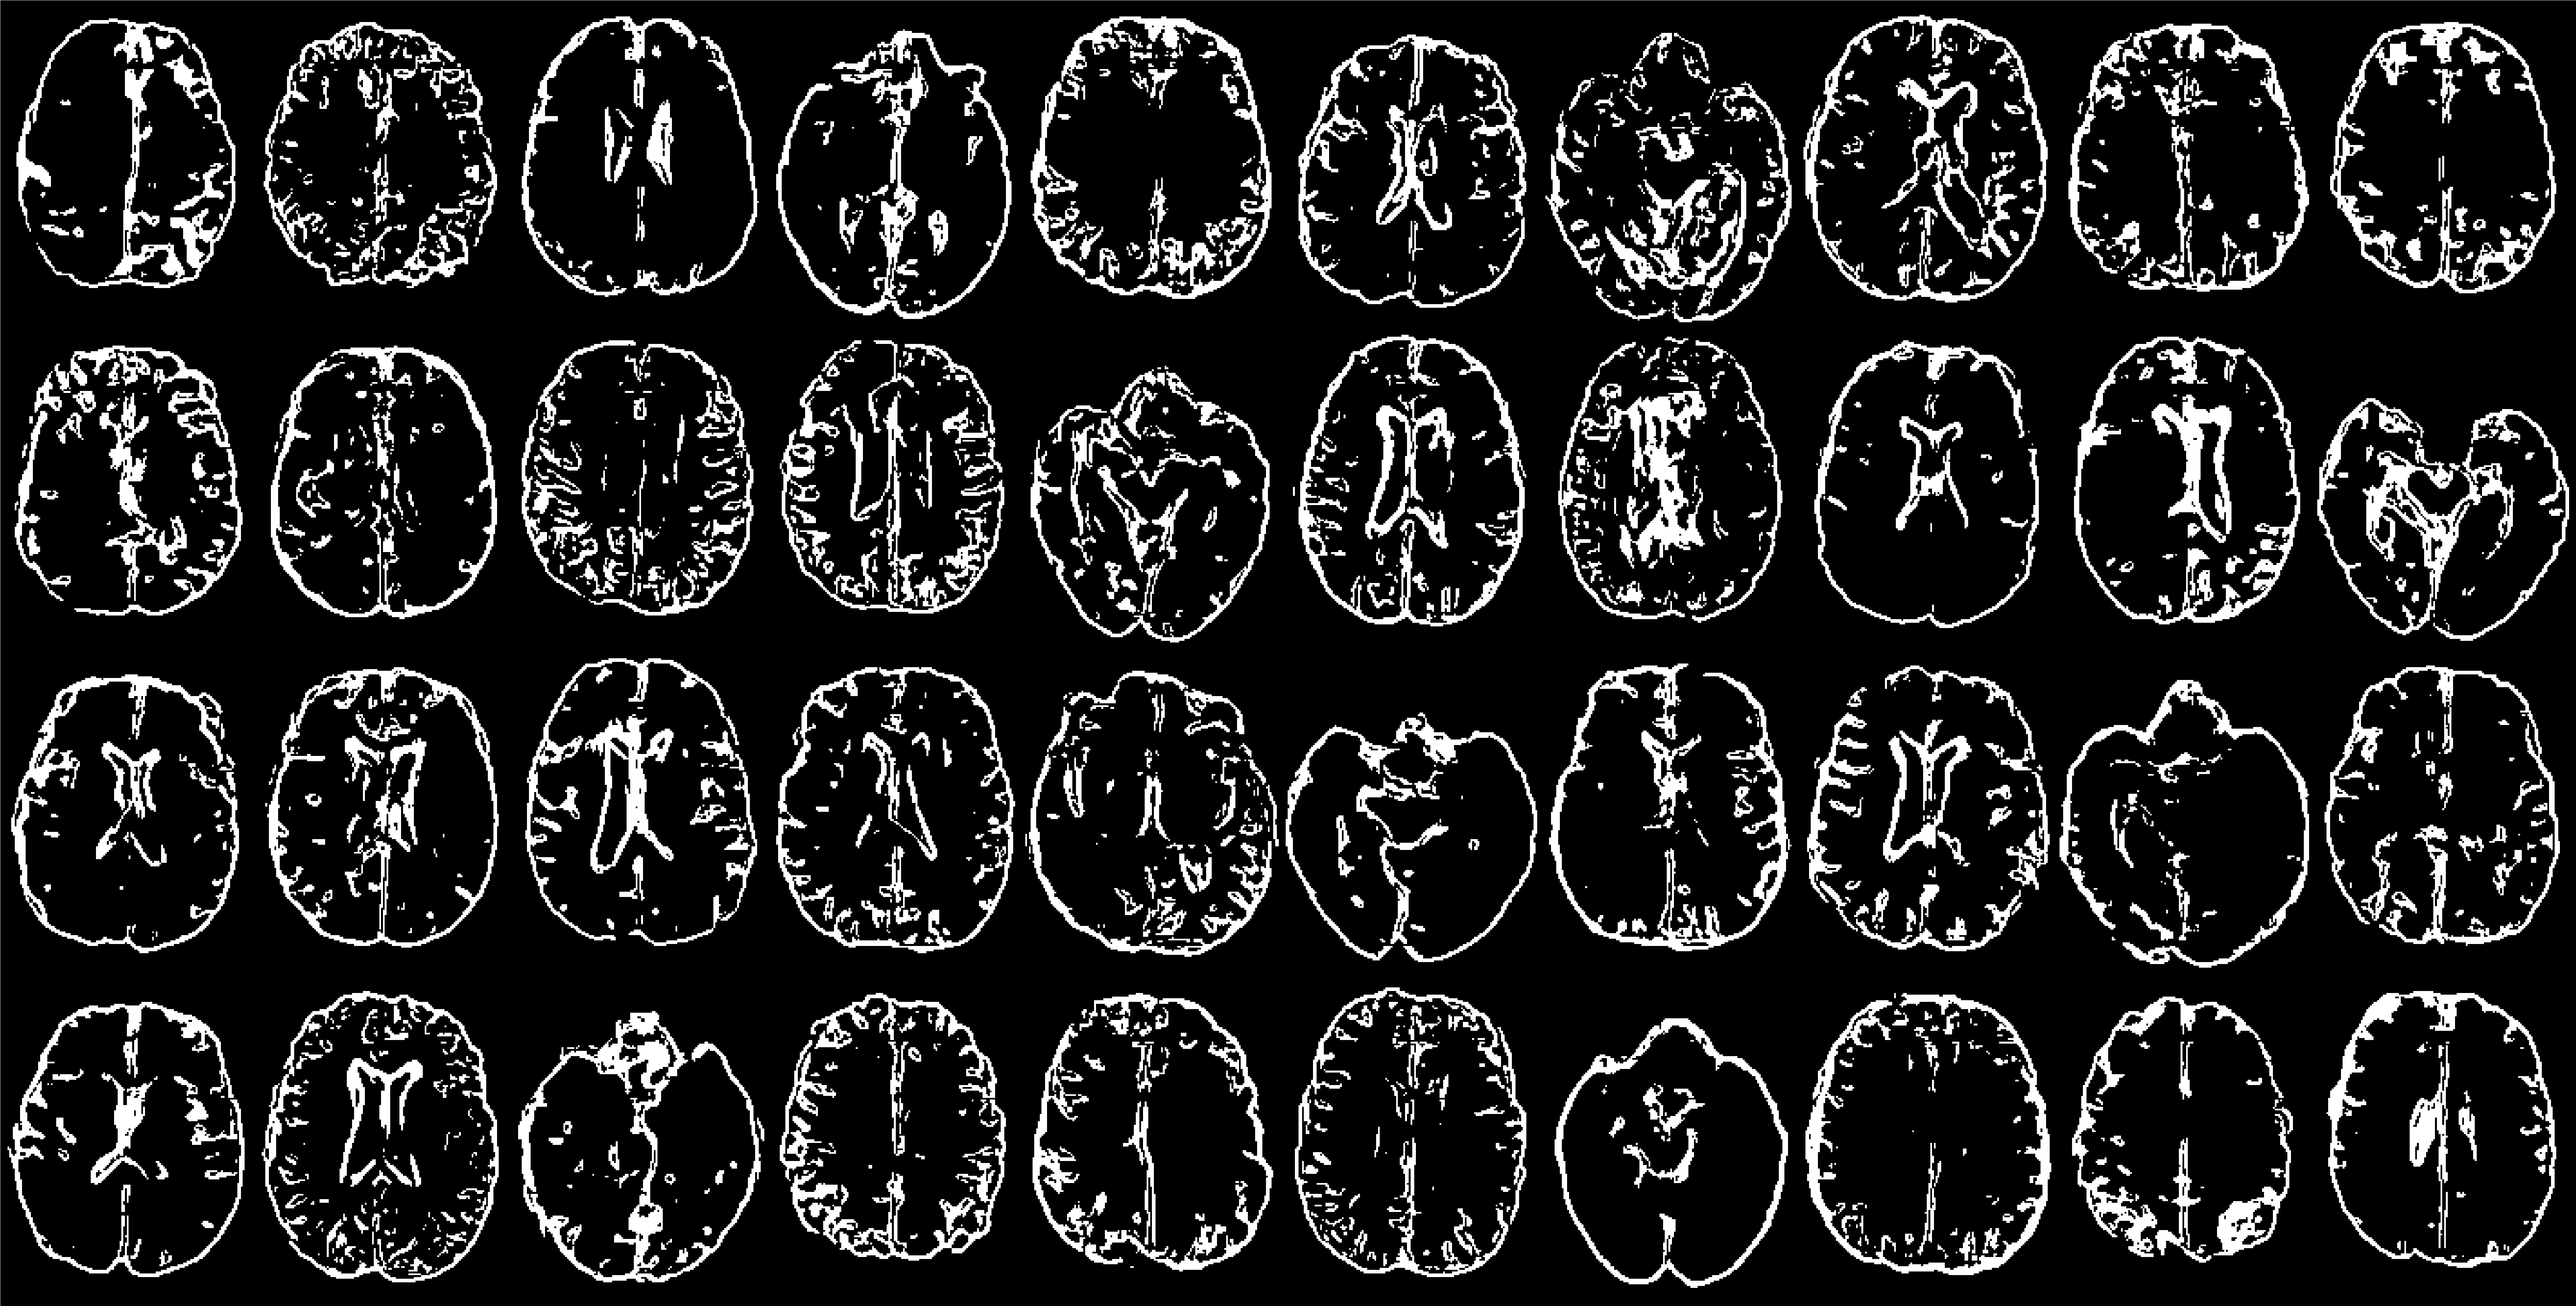
\includegraphics[width=0.95\linewidth]{figures/Fs}
	\caption{Synthetic structural feature maps.}
	\label{generated_f}
\end{figure}
%Fig.~\ref{generated_f} shows the examples of the structural feature map generated from random normal distribution matrix. 
\begin{figure}
	\centering
	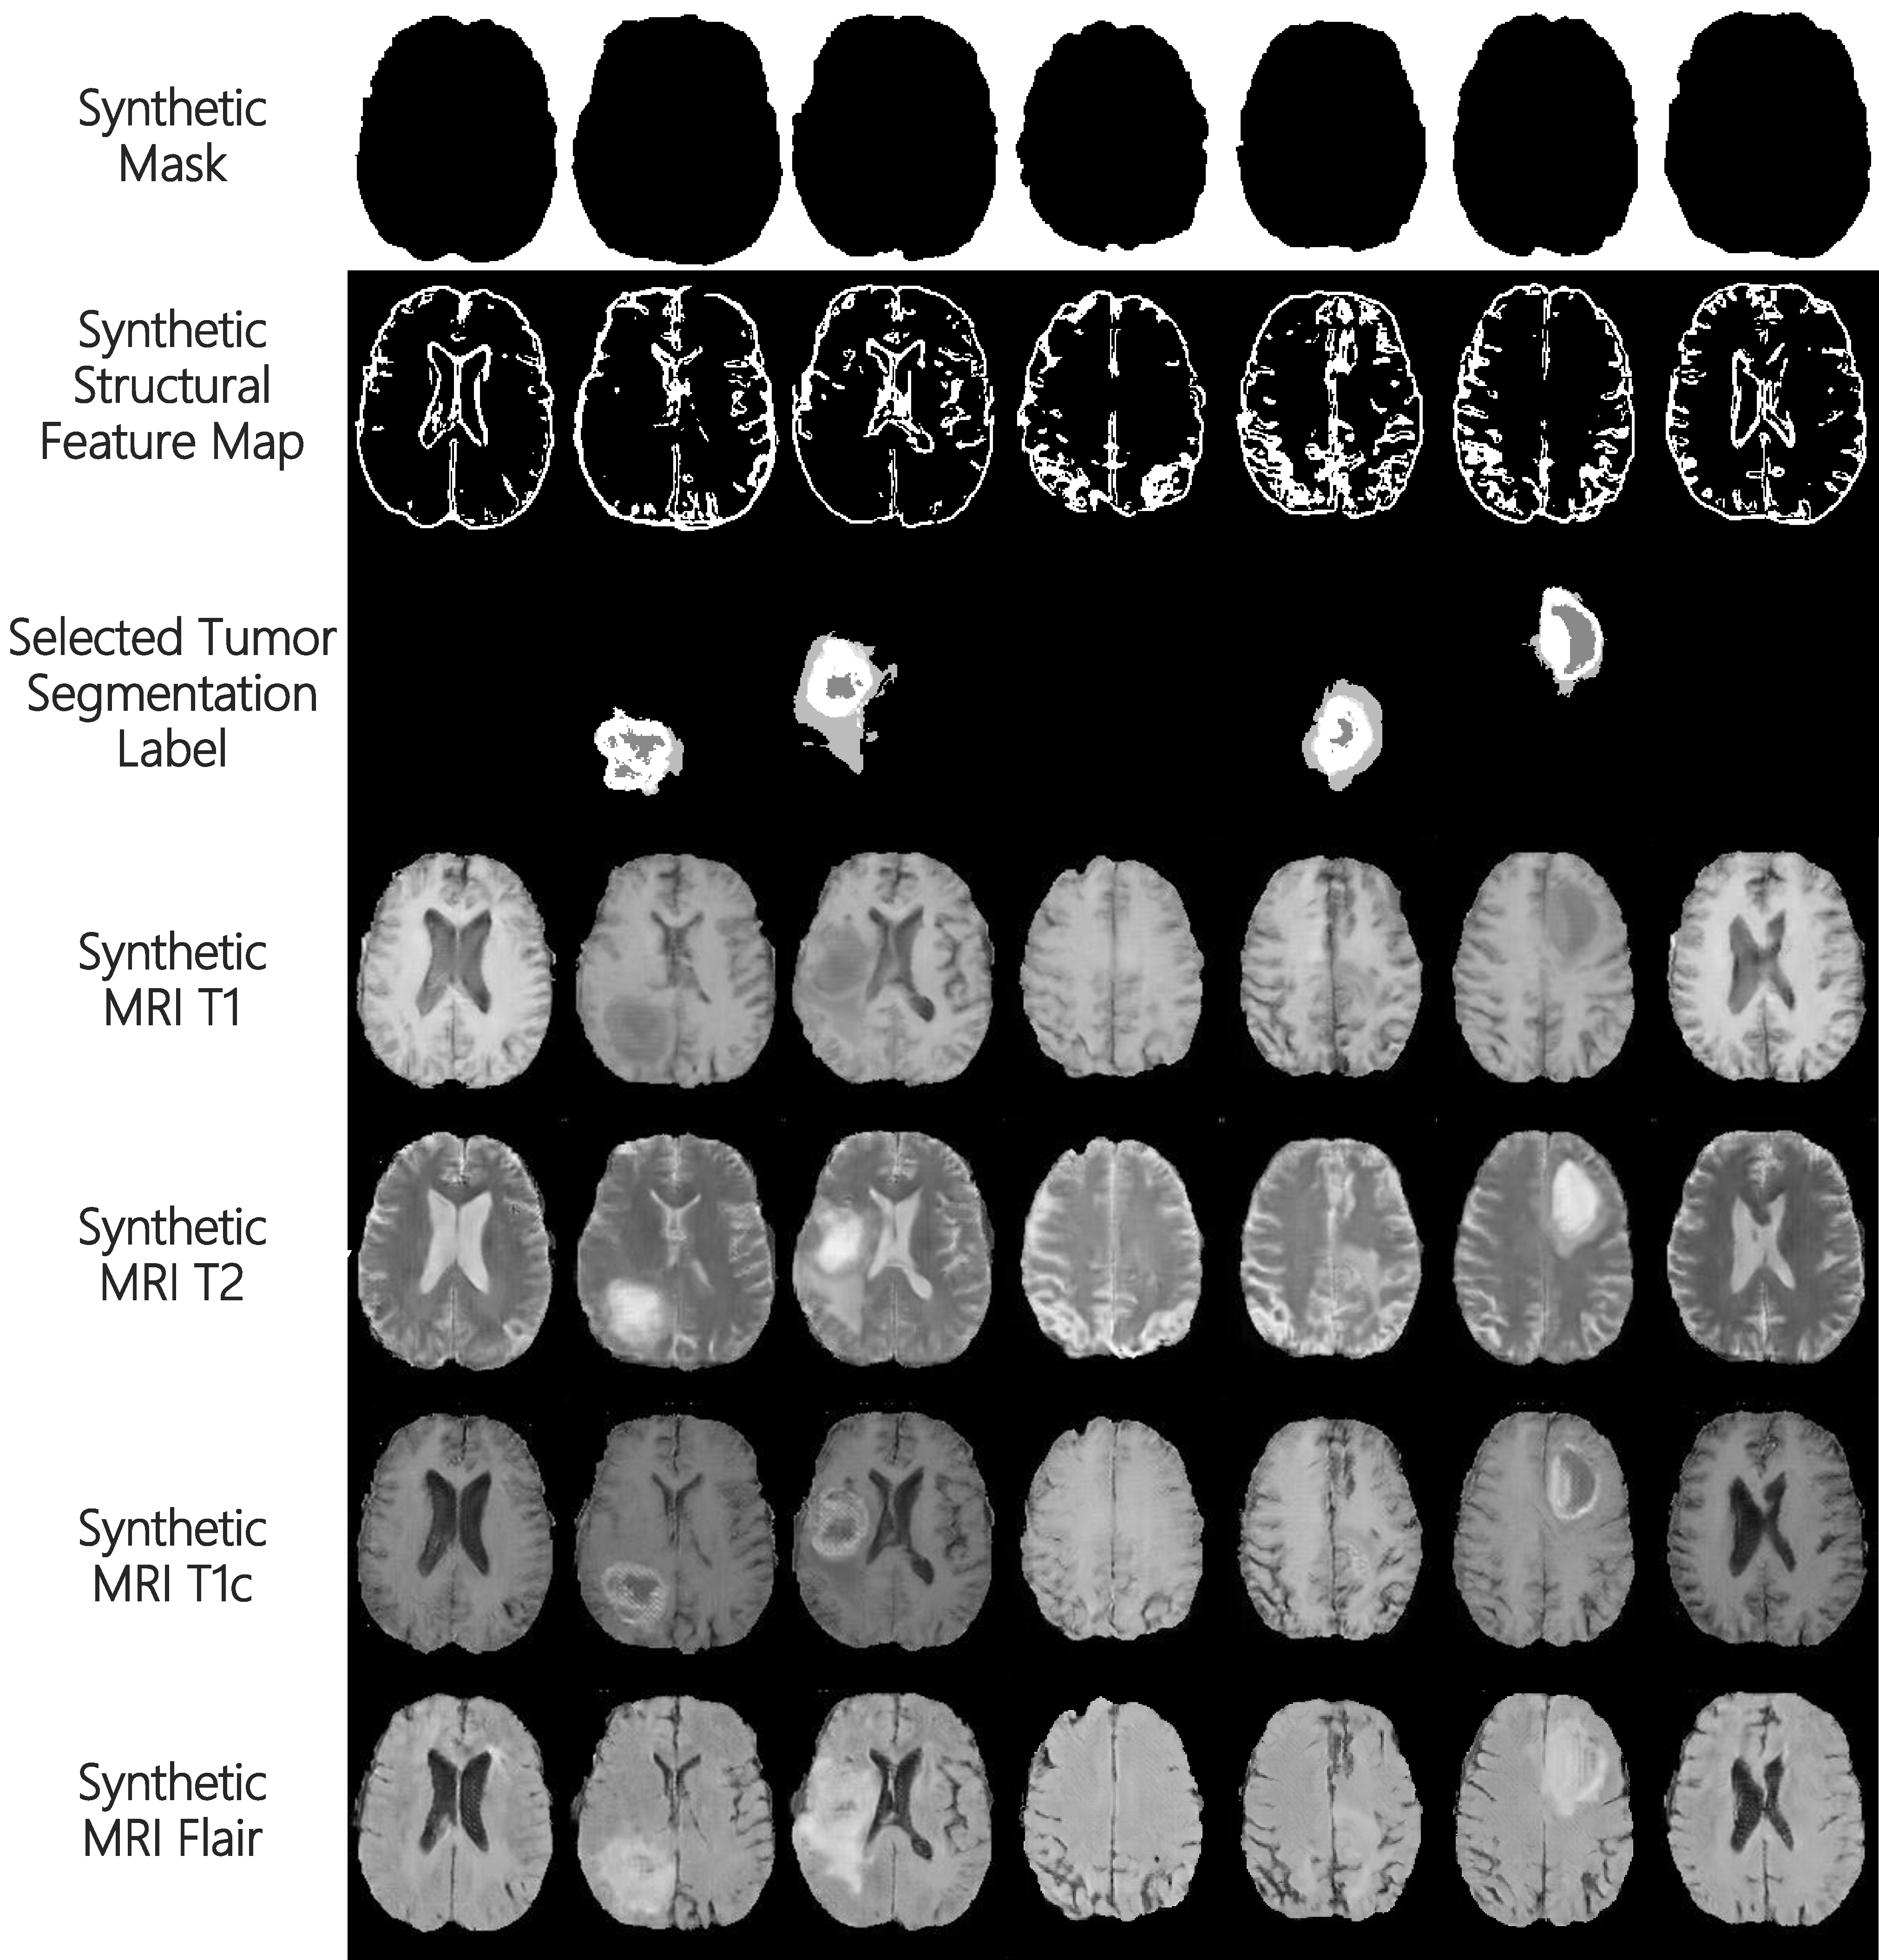
\includegraphics[width=0.98\linewidth]{figures/F_to_MRI}
	\caption{Multimodal MRIs synthesized from structural feature maps and lesion labels.}
	\label{generated_mri}
\end{figure}

\section{CONCLUSION}
In short, we propose a structural feature map extraction method to extract anatomical structure information directly from medical images without training or additional label data.
We propose a structure feature map generation method to generate structural feature maps from multidimensional normal distribution matrixes.
We realize the synthesis of registered multimodal MRI images from a random normal distribution matrix through unsupervised training, which can add the lesion information freely.
We verify that synthetic MRI images can be used as pre-training data or enhanced data for intelligent medical image processing tasks and can significantly improve the generalization ability of the model through lesion segmentation experiments.
\iffalse
In this paper, our contributions are as follows:
\begin{itemize}
	\item We propose a structural feature map extraction method to extract anatomical structure information directly from medical images without training or additional label data.
	\item We propose a structure feature map generation method to generate structural feature maps from multidimensional normal distribution matrixes.
	\item We realize the synthesis of registered multimodal MRI images with corresponding lesion information from structural feature map and randomly selected lesion labels.
	\item We verify that synthetic data can be used as pre-training data or enhanced data for intelligent medical image processing tasks through a number of data availability tests.
\end{itemize}
\fi
%\ack We would like to thank the 
% Quality control editor: Please note that some text appears to be missing in the previous sentence. Please add any missing information.

\bibliography{refer}
\end{document}
%%%%%%%%%%%%%%%%%%%%%%%%%%%%%%%%%%%%%%%%%%%%%%%%%%%%%%%%%%%%%%%%%%%%%%
